% !TeX spellcheck = en_US
\label{sec:concept}

\section{Overall system architecture and services}
\label{sec:concept:sysarchitecture}
\todo{highlight the differences between optimal (proposed) infrastructure and the implementation}
\todo{We vs. I}

Based on the accomplishments of current model repositories (\emph{BioModels database} and \emph{PMR2}), we want to reach further and not only design a concept to simply store multiple versions of a model, but to enrich the version hops with additional information -- more specifically we decided to store deltas between versions, to allow for more specific search queries or analysis of changes between versions.
As base system \masymos was chosen, since it already provides good import methods for both model formats this work focuses on (\sbml and \cellml) and uses \neoj as underlaying database system (cf. Section \ref{sec:background:graph-db:masymos}). The graph-based approach of \neoj allows to store highly interlinked heterogeneous data in a efficient and easily queryable way, making it the perfect tool for storing \sysbio models and deltas of them (cf. Section \ref{sec:background:graph-db:neo4j}).  

Since \masymos was build as an index database for models, it is not possible to reconstruct the \xml model document out of \masymos itself. Consequently all files need to be accessible in another way. For this purpose I choose a static HTTP server, which serves all model files, organized in a specific folder structure. The structure is described in detail in Section \ref{sec:concept:filestorage}.
Said structure is generated by the \modelcrawler, when gathering all model versions from a variety of repositories. As Figure \ref{fig:system-overview} indicates, the \modelcrawler (cf. Section \ref{sec:impl:masymos}) crawls the model files and stores them in the file system, accessible via a HTTP server. Afterwards it sends a request to the \rest API of \masymos, called \morre, which in turn pulls the model from the HTTP server and inserts it into \neoj, using subroutines of the \masymos implementation.

The \modelcrawler in fact is a product of my former activity at the department of \sysbio and Bioinformatics at the University of Rostock, hence it is not directly part of this work. However it is essential for the prototype implementation and therefore describe in Section \ref{sec:impl:modelcrawler}.
\todo{Check if it's ok to say this.}

Once all desired model versions are imported into \masymos via the \morre interface, an  asynchronous task will generate all deltas. The execution of this task may be triggered, using a \rest endpoint from the to be implemented diff \rest interface. Alternatively this task can be activated periodically by a cron job or by a database trigger, in case a new model version is inserted.
However, when a generic diff-generation-task is triggered, another task will automatically started beforehand. This task searches for direct version hops without a delta and submits a diff-generation-task for each of them. 
The actual task generating the delta will fetch the \xml documents of both versions from the HTTP server and send them to \bives to compare those versions. The result is consequently analyzed, translated into a graph structure (cf. Section \ref{sec:concept:dbmodel}), and inserted into the database.

As shown in Figure \ref{fig:system-overview}, the main part of the implementation splits into two projects: the diff \rest plugin and the \masymos-diff plugin. This separation is intended to mimic the project structure of \masymos itself, which was meant to separate public APIs from the actual implementation, so it is easy to build multiple front ends, for instance a Command Line Interface (CLI) for easier debugging during development phases. Consequently I followed this example as well and also used a CLI during development.

\begin{figure}[h]
	\centering
	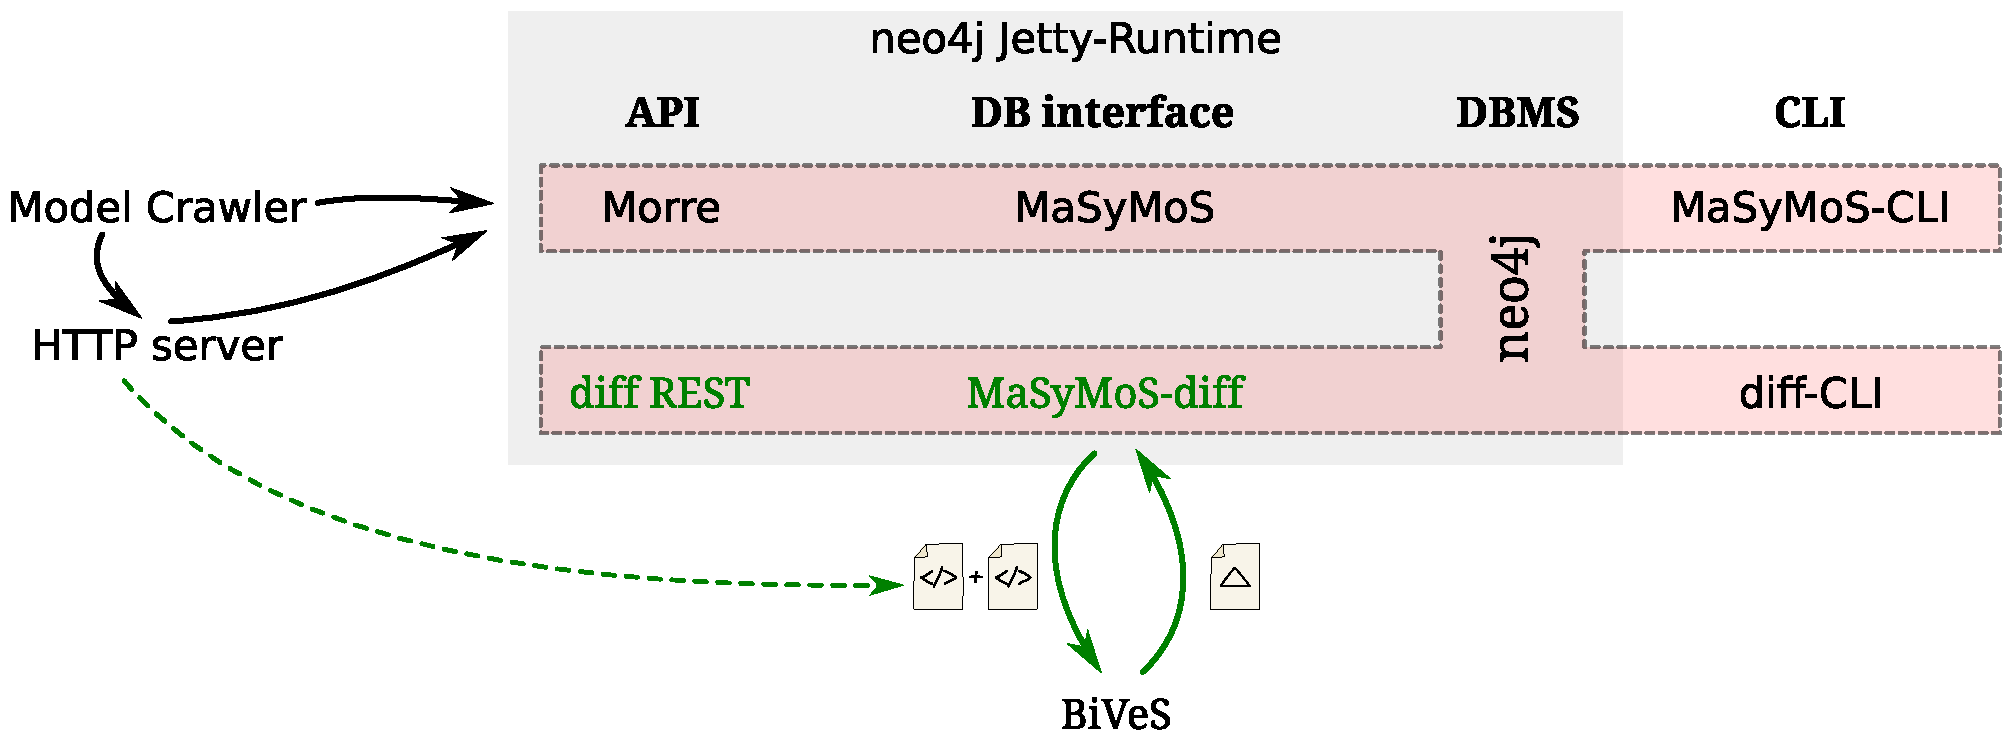
\includegraphics[width=\textwidth]{resources/system-overview-matrix.pdf}
	\caption[Infrastructure overview]{The \textbf{Infrastructure overview} shows the intended system architecture of \masymos \neoj and additional services. New implementations are displayed in green, whereby the parts directly extending \neoj are located in the red box.}
	\label{fig:system-overview}
	\todo{actually add the CLI to the figure}
	\todo{Write \modelcrawler with space in figure}
\end{figure}

\section{Database model and storage decisions}
\label{sec:concept:dbmodel}
\begin{comment}
\begin{itemize}
\item extension to database model cf. \ref{fig:db-model}
	\subitem linking version
	\subitem storing differences
\item decisions on storage model
	\subitem storing each version full (no delta-storage)
	\subitem each version is aware to the search index
	\subitem diff still enables for analysis of changes
	\subitem higher storage consumption
\item extended storage model
\end{itemize}
\end{comment}
% description of ER model
\todo{intro sentence}
Figure \ref{fig:db-er-model} shows the proposed database schema as ER model. To reduce complexity and redundancy, the storage structure of models in \masymos is simplified, shown on the left hand side of the figure. Further the \comodi ontology (cf. Section \ref{sec:background:onto:comodi}) is not remodeled, but instead represented as generic \texttt{OntologyTerm}.

\todo{Add color to the diagram, to ease explanation}

The schema is organized around a \texttt{Diff} entity linking two \texttt{Document} entities, which represents a (XML-)document containing a model. If these \texttt{Documents} contain two consecutive versions of a model, they are linked with a \texttt{has\_successor} and a \texttt{has\_predecessor} relation. These relations are maintained by \masymos itself, whereby the interlink, created to anchor a diff, is expressed via the \texttt{has\_diff} relation, which can be declared in two roles: \emph{source} and \emph{destination}. I decided to use these terms in order to prevent confusion regarding the time line of the model versions, since \bives also does not discriminate any temporal information.
These 2-hop relations do not necessarily need to span between two consecutive versions.
Instead I decided, that for a standard setup it might be less useful to store deltas between every possible combination of versions, since this would consume unreasonable amount of storage.
Further deltas can be concatenated, so it does not take any significant computational effort to generate a diff for larger version steps out of consecutive deltas.

Every \texttt{Diff} entity links to one, multiple, or none (in case of an empty delta) \texttt{DiffEntry} entities via the \texttt{has\_entry} relation.  
A \texttt{DiffEntry} can be either a \texttt{DiffInsert},  \texttt{DiffDelete}, \texttt{DiffMove} or a \texttt{DiffUpdate} entity, following the terms used by \bives \citep{Scharm2015} and \comodi \citep{Scharm2016}.

Each \texttt{DiffEntry} represents a difference detected by \bives \citep{Scharm2015} and links to at least one \texttt{ModelEntity} via either \texttt{is\_source}, \texttt{is\_destination}, or both relations, depending on the type of the change.
For instance a \texttt{DiffInsert} links to a \texttt{ModelEntity} of the \emph{destination} with an \texttt{is\_destination} relation.
In contrast a \texttt{DiffDelete} links to the \emph{source} version with an \texttt{is\_source} relation to a \texttt{ModelEntity}. Whereby \texttt{DiffMove} and \texttt{DiffUpdate} entities use both relations: \texttt{is\_source} to link to the \emph{source}, and \texttt{is\_destination}, to link to the \emph{destination} version.

Additionally a \texttt{DiffEntry} can link to an \texttt{OntologyTerm}. Ontology terms are hierarchically structured, but not modeled in this ER model. Those terms are currently taken from the \comodi ontology \citep{Scharm2016}, to describe the nature of changes (cf. Section \ref{sec:background:onto:comodi}).

\todo{add table (or similar) of all entities and relations in the appendix}
\todo{make visible, that ER model is just a sub-ER}

\todo{Add argument, that \masymos is only search index and does not allow for model reconstruction from the database}
\todo{mention, what is stored in attributes}

\begin{figure}
	\centering
	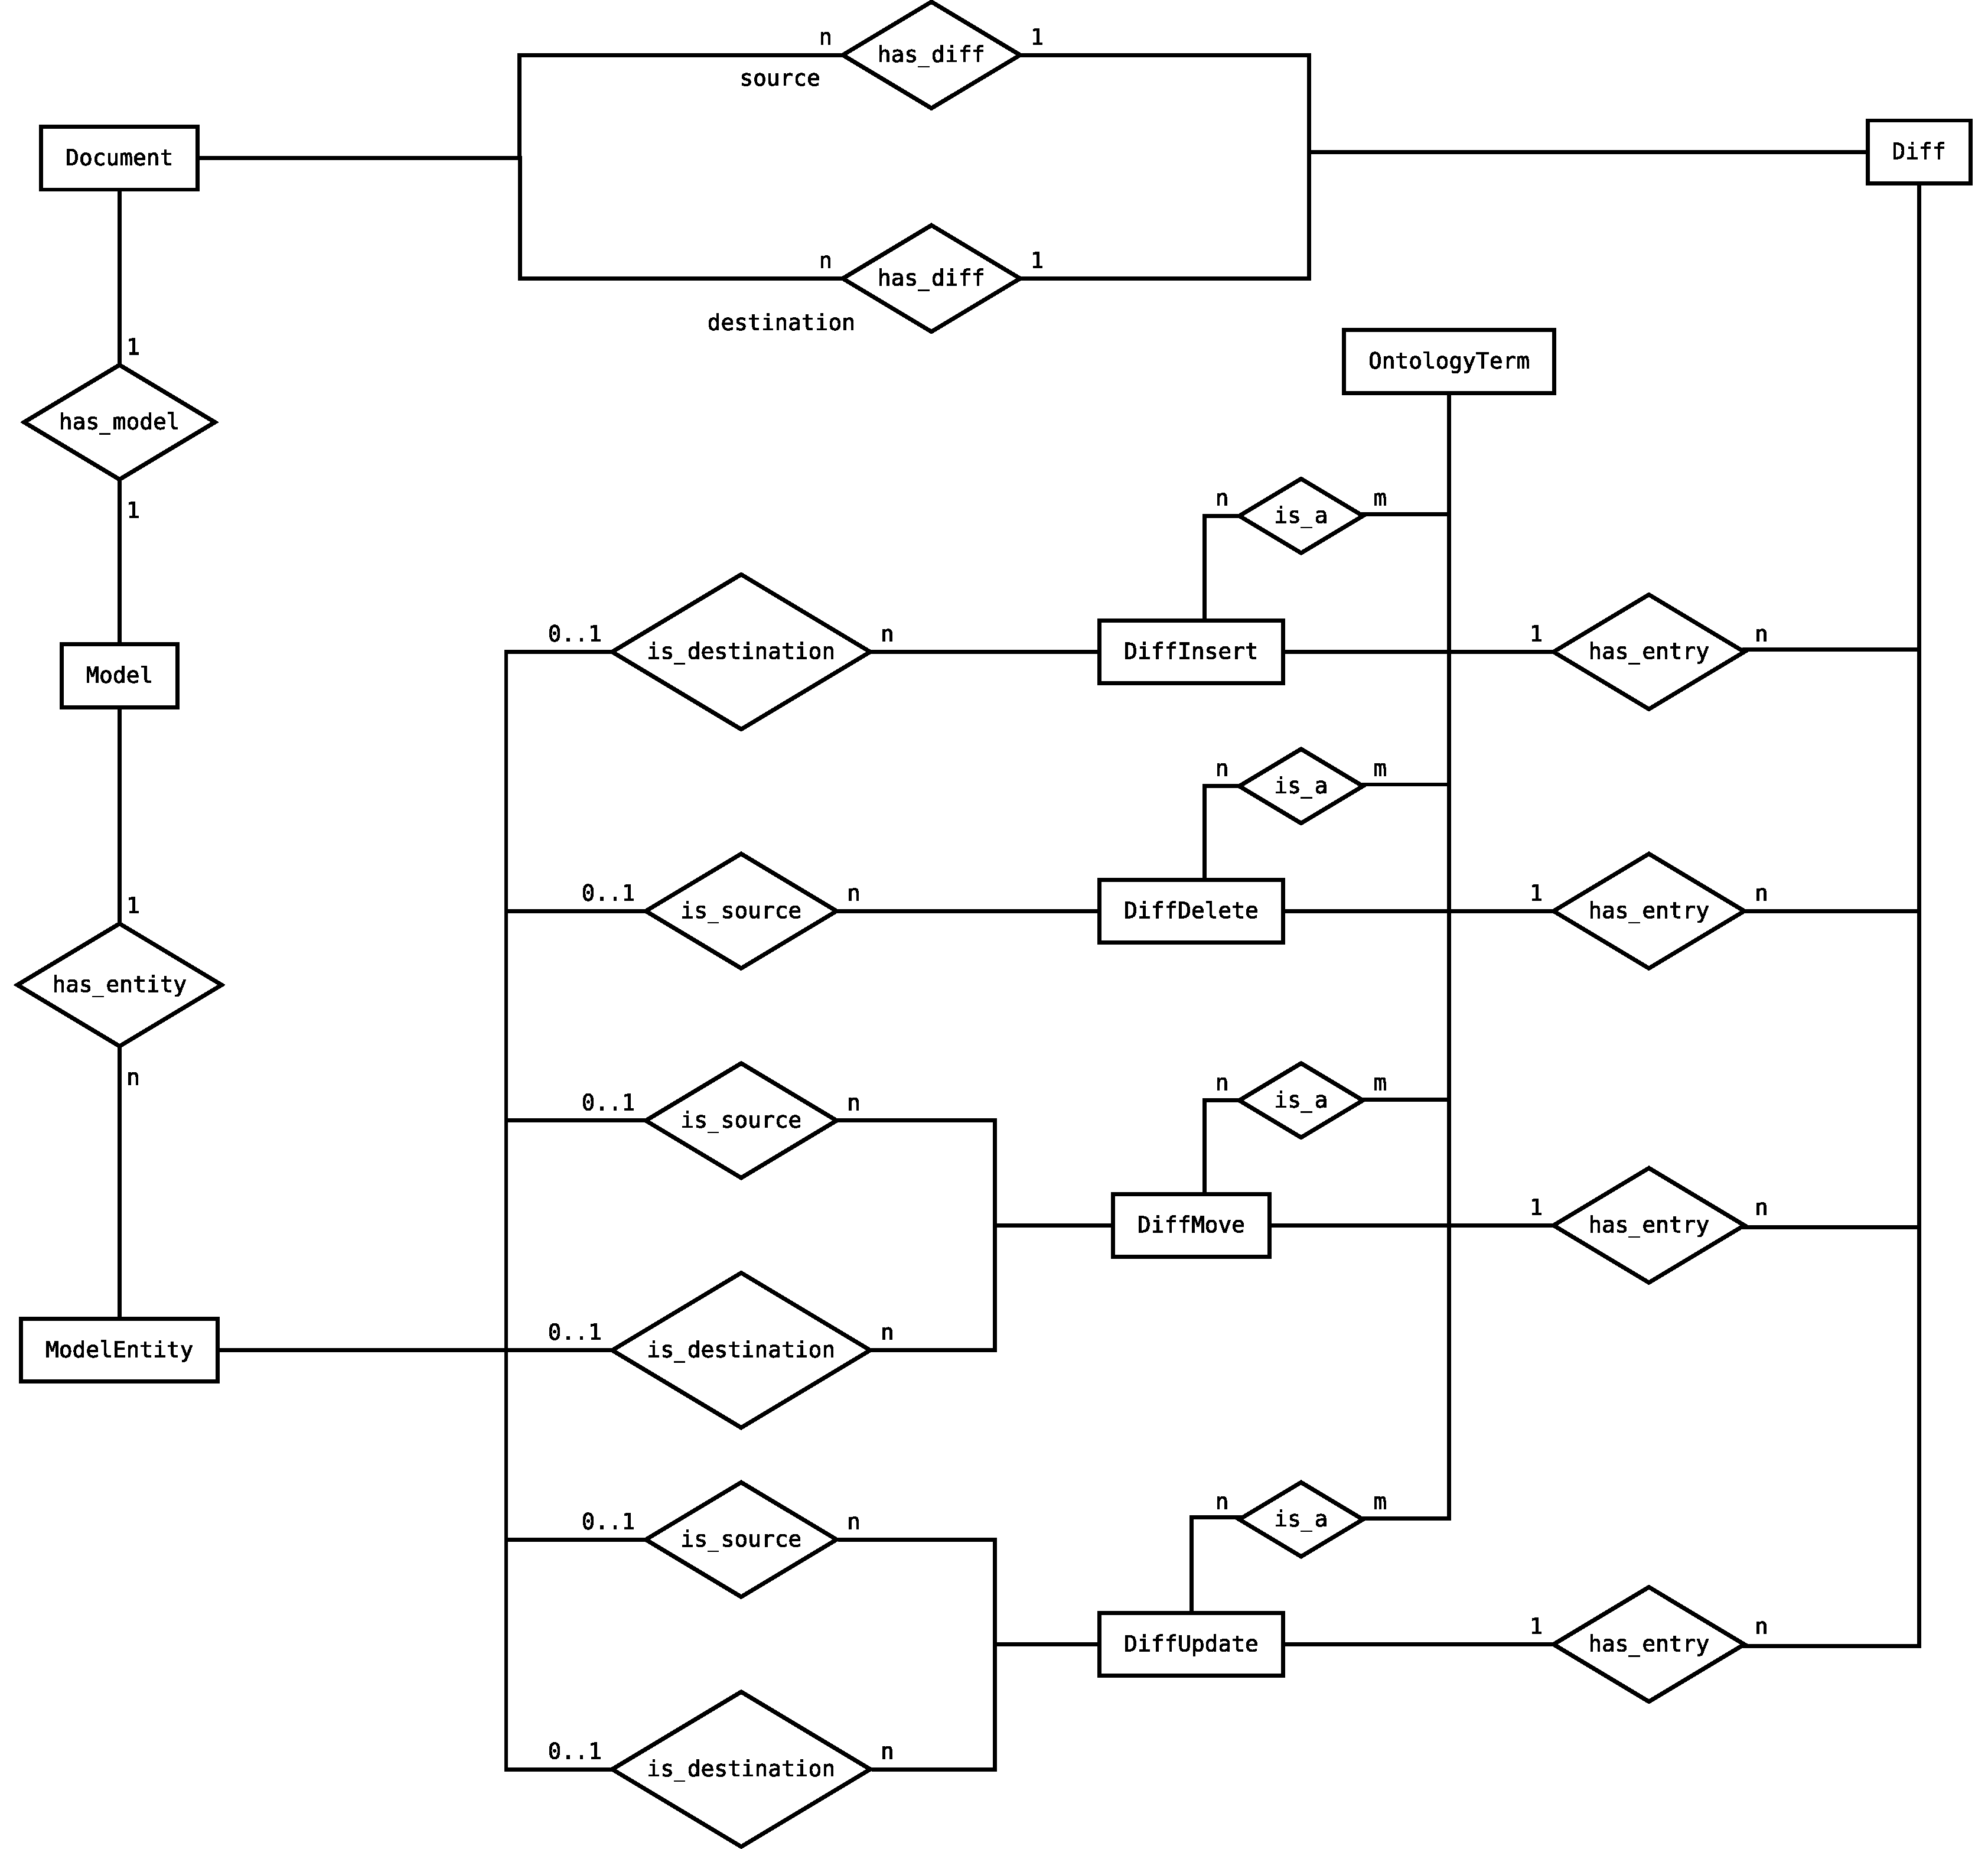
\includegraphics[width=\textwidth]{resources/db-concept-er.pdf}
	\caption{ER model of the proposed database schema}
	\label{fig:db-er-model}
\end{figure}

%\begin{figure}[h]
%	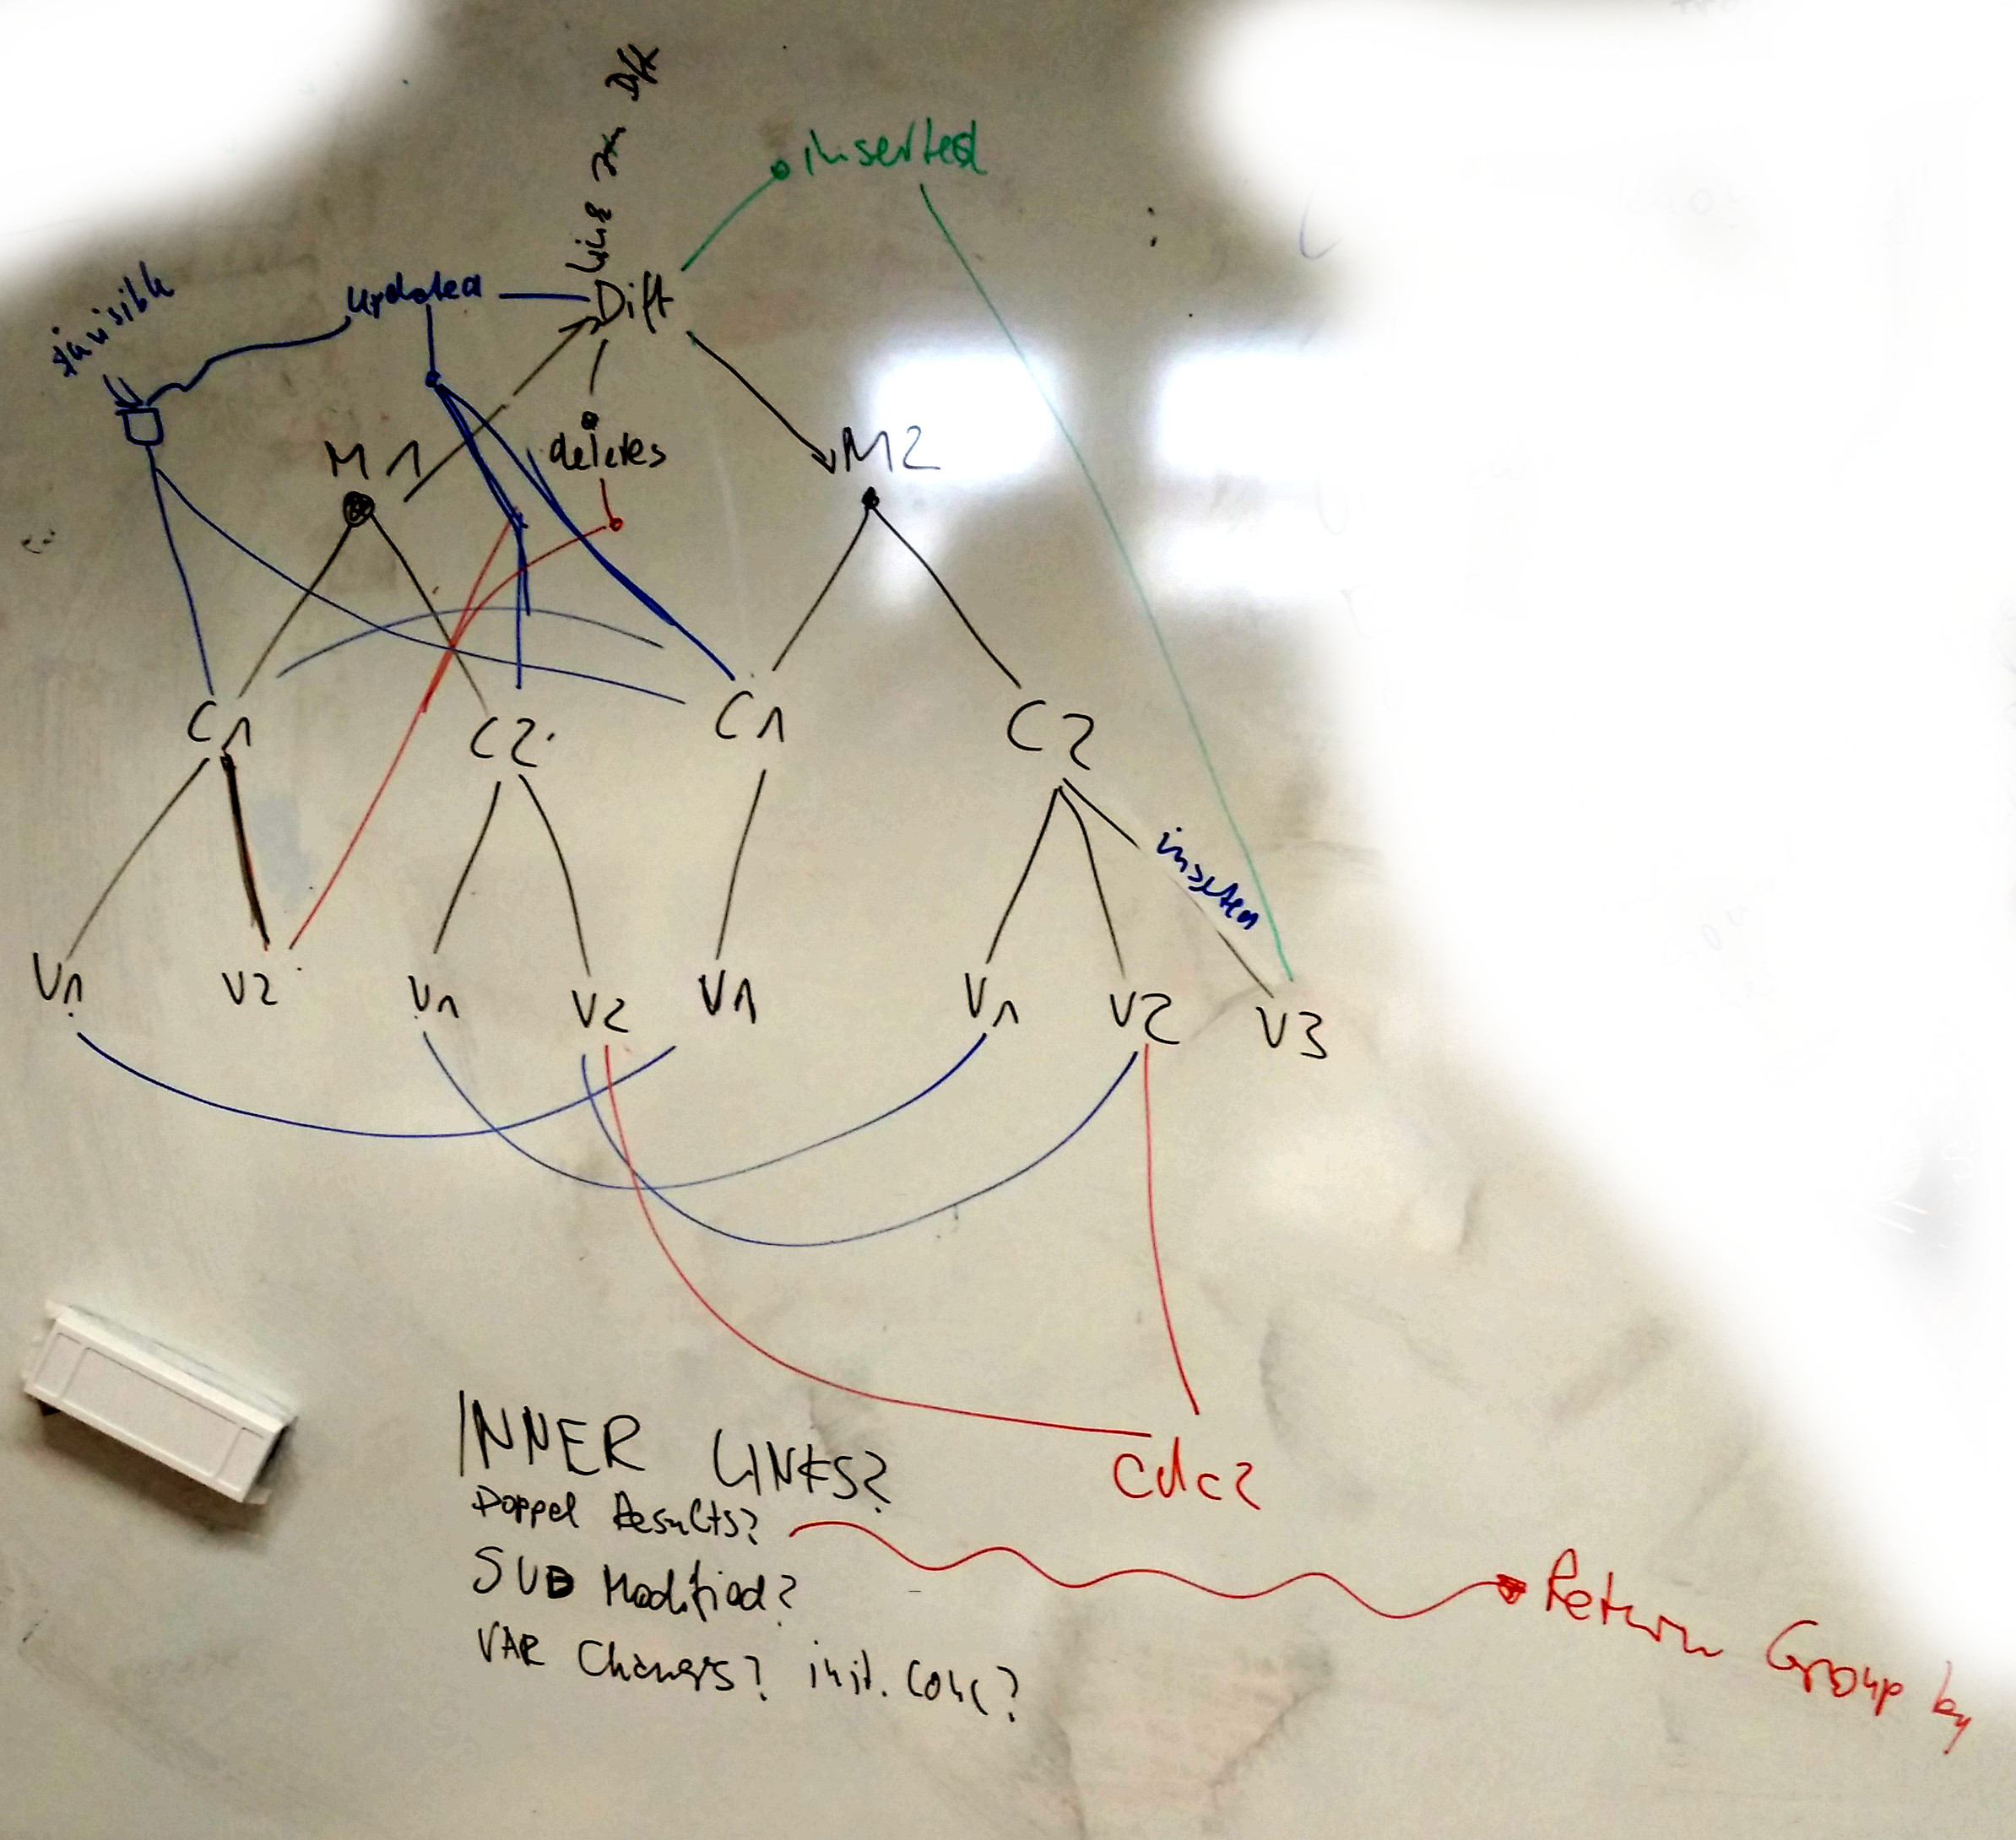
\includegraphics[width=\textwidth]{resources/db_structure.jpg}
%	\caption{Proposed database structure}
%	\label{fig:db-model}
%\end{figure}

\section{The HTTP file server}
\label{sec:concept:filestorage}

The concept of having a HTTP daemon serving all original model files in the \masymos database, as introduced in Section \ref{sec:concept:sysarchitecture}, was originally developed during work as student assistant at the Department of \sysbio and Bioinformatics at the University of Rostock, but was improved in preparation of this work.

The file structure, created by the \modelcrawler, is organized around the concept of a \texttt{fileId} and a \texttt{versionId}. First one is uniquely identifying one (model) file over time, whereby the \texttt{versionId} has to be unique within the specific history of this file. Together they point to one version of a model and therefore form a primary key.
When designing this concept, we needed to take special care for the \cellml Model Repository PMR2 (cf. Section \ref{sec:background:modelrepo}), because the \cellml provides an import feature for submodels or unit definition and consequently one model may consist of a lot of different files. In order to not break the import directives, the relative positions of these files need to be recreated. As a result the \texttt{fileId}, represented as URN, is split into 2 parts separated by an explanation mark (\texttt{!}). The first part points to the \emph{workspace} of the model, meaning the folder/git repository containing all relevant files, and is therefore equal for all files belonging into one workspace. The second part indicates the relative position of the file, \emph{within} the workspace.
Consequently a valid \texttt{fileId} would for instance look like this:\\ \texttt{urn:model:models.cellml.org:workspace:novak\_tyson\_1997:!:novak\_tyson\_1997.cellml}\\
In this example \texttt{urn:model} is the prefix, \texttt{models.cellml.org:workspace:novak\_tyson\_1997} the workspace, and \texttt{novak\_tyson\_1997.cellml} the path of the actual model file within the workspace. In addition, the separation marker could also be concatenated with the \texttt{versionId}, using one URN to describe on specific version of a model. This extended URN format can also be directly converted into an absolute URL, pointing to a model file, if the address of the HTTP server is known.
Given the \texttt{versionId} in above mentioned example would be \texttt{3614b6d39b91d78e0038bbd113814686c316616b}, and assuming the HTTP server is available under the imaginary host \texttt{models.example.org}, the following URL could be used to access the actual file:\\
\texttt{http://models.example.org/models.cellml.org/workspace/novak\_tyson\_1997/3614b6d39b91d78e0038bbd113814686c316616b/novak\_tyson\_1997.cellml}

Additionally the \modelcrawler also creates files in the root of the workspace path with additional information about the origin, the date, and crawled date of each version.
The purpose of these \json encoded files is to ensure that basic provenance information are also available, if the \masymos database is unavailable.

